%%%%%%%%%%%%%%%%%%%%%%%%%%%%%%%%%%%%%%%%%%%%%%%%%%%%%%%%%%%%%%%%%%%%%%%%%%%
%% This file is part of the book
%%
%% Algorithmic Graph Theory
%% http://code.google.com/p/graph-theory-algorithms-book/
%%
%% Copyright (C) 2009--2011 Minh Van Nguyen <nguyenminh2@gmail.com>
%%
%% See the file COPYING for copying conditions.
%%%%%%%%%%%%%%%%%%%%%%%%%%%%%%%%%%%%%%%%%%%%%%%%%%%%%%%%%%%%%%%%%%%%%%%%%%%

\documentclass{article}

\usepackage{tikz}
\usepackage{tkz-berge}  %% for drawing combinatorial graphs
\usetikzlibrary{external}
\tikzexternalize{routing-network}

\begin{document}

\begin{figure}
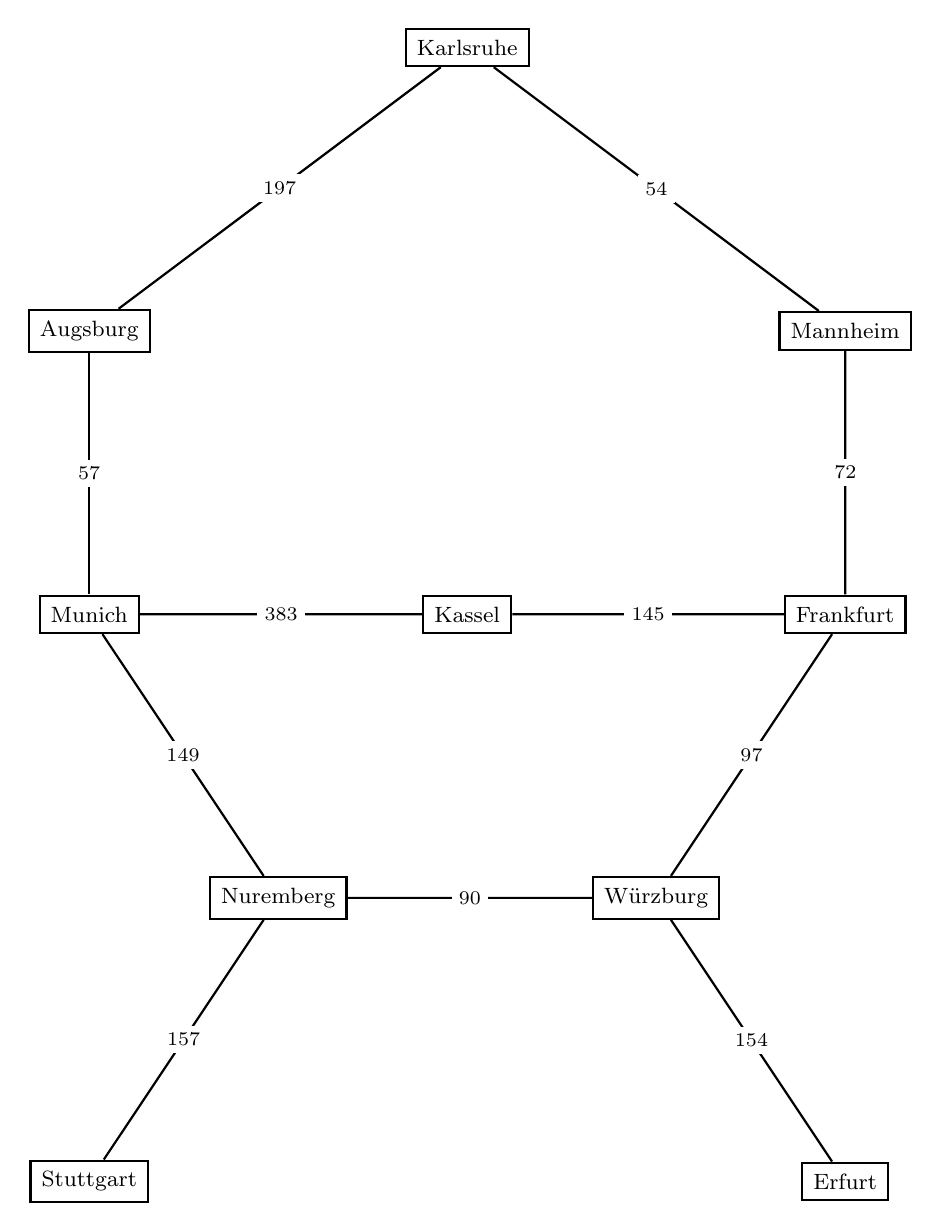
\begin{tikzpicture}
[nodeDecorate/.style={shape=rectangle,inner sep=4pt,draw,thick},%
  scale=1.2]
%% nodes or vertices
\foreach \nodename/\x/\y in {
  Stuttgart/0/0, Erfurt/8/0, Nuremberg/2/3, Munich/0/6, Frankfurt/8/6,
  Kassel/4/6, Augsburg/0/9, Mannheim/8/9, Karlsruhe/4/12}
{
  \node (\nodename) at (\x,\y) [nodeDecorate] {\footnotesize\nodename};
}
\node (Wurzburg) at (6,3) [nodeDecorate] {\footnotesize W\"urzburg};
%% edges or lines
\tikzstyle{EdgeStyle}=[-,thick]
\tikzstyle{LabelStyle}=[fill=white]
\foreach \startnode/\endnode/\distance in {
  Stuttgart/Nuremberg/157, Erfurt/Wurzburg/154,
  Nuremberg/Wurzburg/90, Nuremberg/Munich/149,
  Wurzburg/Frankfurt/97, Munich/Kassel/383,
  Frankfurt/Kassel/145, Munich/Augsburg/57,
  Frankfurt/Mannheim/72, Augsburg/Karlsruhe/197,
  Mannheim/Karlsruhe/54}
{
  \scriptsize
  \Edge[label=$\distance$](\startnode)(\endnode)
}
\end{tikzpicture}
\end{figure}

\end{document}
